\documentclass[10pt,a4paper]{article}
\usepackage{geometry}
 \geometry{
 a4paper,
 total={170mm,257mm},
 left=20mm,
 top=20mm,
 }


\usepackage[utf8]{inputenc}
\usepackage[spanish]{babel}
\usepackage{graphicx}
\usepackage{wrapfig}
\usepackage{amssymb, amsmath}
\usepackage{tikz}
\usepackage{enumitem}

\title{Subestaciones y centros de transformación}
\author{MakerGarage}
\date{Mayo 2021}


\setlength{\parindent}{0cm}


\renewcommand{\thesubsection}{\Roman{subsection}}
\renewcommand{\thesubsubsection}{\alph{subsubsection})}

\begin{document}

\maketitle
\newpage
\tableofcontents
\newpage
\section{Problemas}
\subsection{Intensidad en alta tensión}
$$
I_p = \frac{S}{\sqrt{3} \cdot U_p} [A]
$$
Donde:
\begin{itemize}
    \item S es potencia aparente en kVA
    \item $U_p$ \text{es la tensión del primario en kV}
\end{itemize}
\subsection{Intensidad en baja tensión}
$$
I_s = \frac{S}{\sqrt{3} \cdot U_s} [A]
$$
Donde:
\begin{itemize}
    \item S es potencia aparente en kVA
    \item $U_s$ \text{es la tensión del secundario en kV}
\end{itemize}

\subsection{Intensidad de cortocircuito en alta tensión}
$$
I_{ccp} = \frac{S_{cc}}{\sqrt{3} \cdot U_p} [A]
$$
Donde:
\begin{itemize}
    \item $S_{cc}$ es potencia aparente de cortocircuito en kVA
    \item $U_p$ \text{es la tensión del primario en kV}
\end{itemize}
\subsection{Intensidad de cortocircuito en baja tensión}
$$
I_{ccs} = \frac{ S}{\sqrt{3} \cdot U_s \cdot \frac{U_{cc}\%}{100} } [A]
$$
Donde:
\begin{itemize}
    \item S es potencia aparente en kVA
    \item $U_s$ \text{es la tensión del secundario en kV}
    \item $U_{cc}\%$ Tensión de cortocircuito en \%
\end{itemize}
\newpage
\subsection{Dimensionado del embarrado}
\subsubsection{Comprobación por densidad de corriente}
$$
d_{corriente} = \frac{I_p}{S}[\frac{A}{mm^2}]
$$
Donde:
\begin{itemize}
    \item $I_p$ [A]
    \item S Sección en $mm^2$
\end{itemize}

\subsubsection{Comprobación por solicitación electrodinámica}
$$
\sigma \operatorname{máx} \geq\left(\operatorname{Iccp}^{2} \cdot L^{2}\right) /(60 \cdot d \cdot W)
$$
Donde:
\begin{itemize}
    \item $I_{ccp}$ Intensidad permanente de cortocircuito trifásico[kA]
    \item L Separación longitudinal entre apoyos [cm]
    \item d  Separación entre fases[cm]
    \item W  Módulo resistente de los conductores[$cm^3$]
\end{itemize}

\subsubsection{Comprobación por solicitación térmica a cortocircuito}
$$
\text { Ith }=\alpha \cdot \mathrm{S} \cdot \sqrt{ \Delta \mathrm{T} / \mathrm{t}}) [A]
$$
\begin{itemize}
    \item $\alpha$ 13 para el cobre
    \item S sección del embarrado en $mm^2$
    \item $\Delta \mathrm{T}$ Elevación o incremento máximo de temperatura 150ºC para Cu
    \item t tiempo del cortocircuito  en s
    
\end{itemize}
\newpage
\section{Teoría}
Todos los centros de transformación disponen de:
\begin{itemize}
    \item Celda de entrada
    \item Celda de salida
    \item Fusible trafo (si es privado no la instalan y corre a cargo del usuario)
    
    \item En caso de ser propiedad privada se añaden
    \begin{itemize}
        \item Celda de entrega
        \item Celda de protección general
        \item Celda de protección del trafo (en caso de ser 2 ya que la general solo vale par 1 trafo)
        \item Celda de medida
    \end{itemize}
\end{itemize}
\section{Tipos de CT}
\begin{center}
    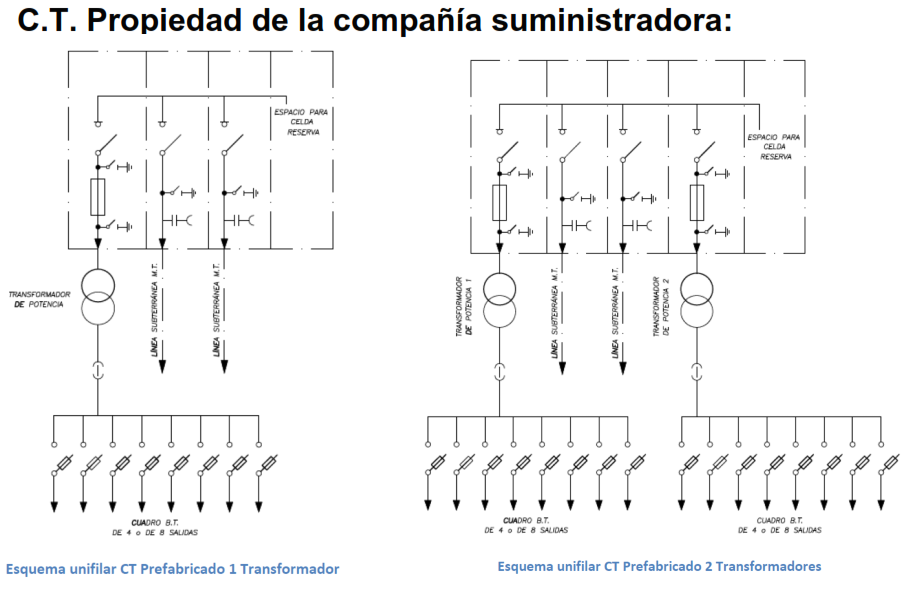
\includegraphics[scale = 0.6]{1.png}
    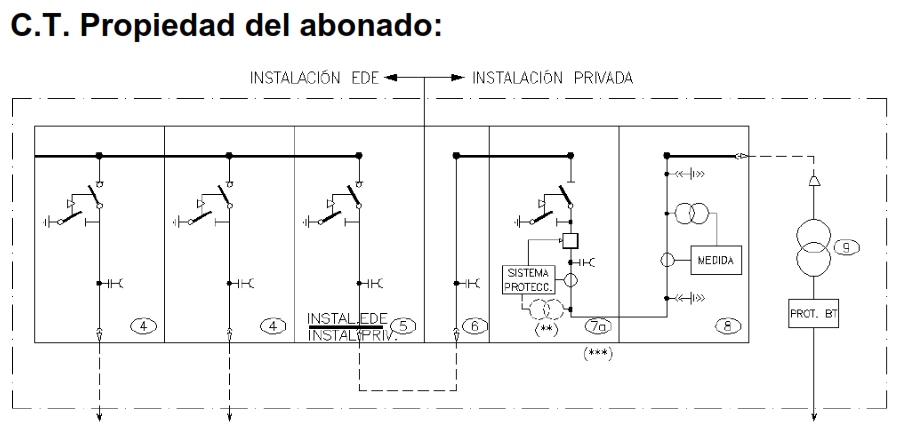
\includegraphics[scale = 0.6]{2.png}
\end{center}

\section{Tipos de Subestaciones}
\begin{center}
    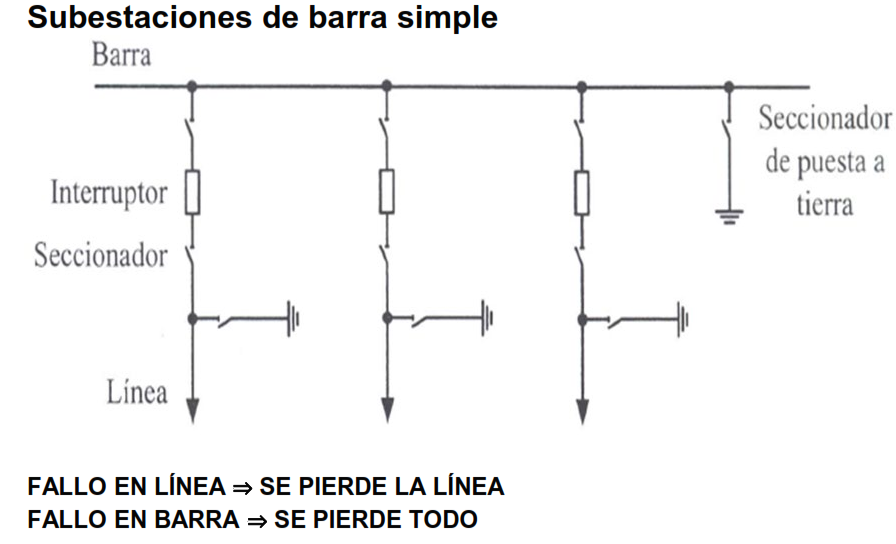
\includegraphics[scale = 0.6]{3.png}
    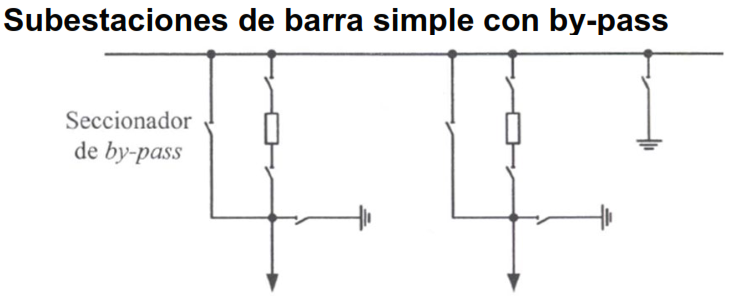
\includegraphics[scale = 0.6]{4.png}
    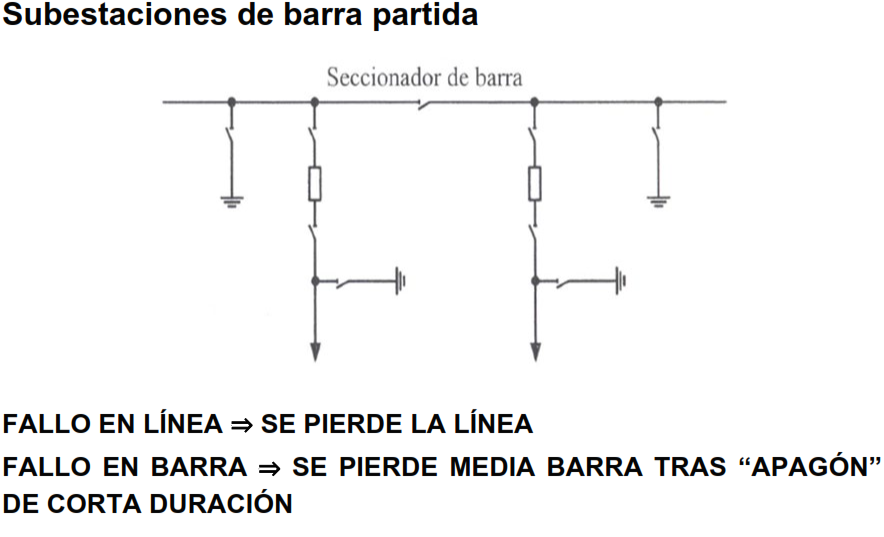
\includegraphics[scale = 0.6]{5.png}
    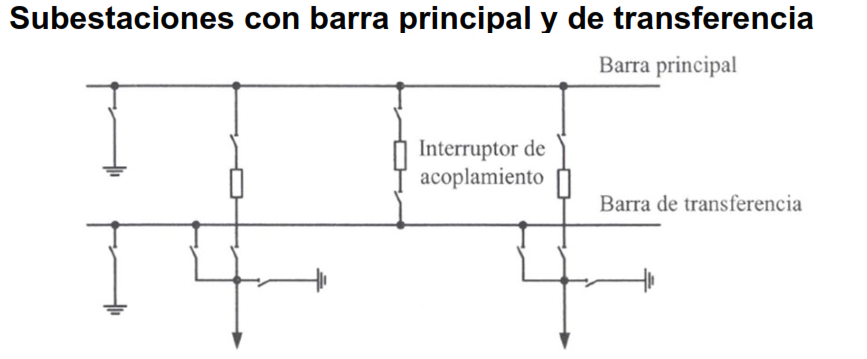
\includegraphics[scale = 0.6]{6.png}
    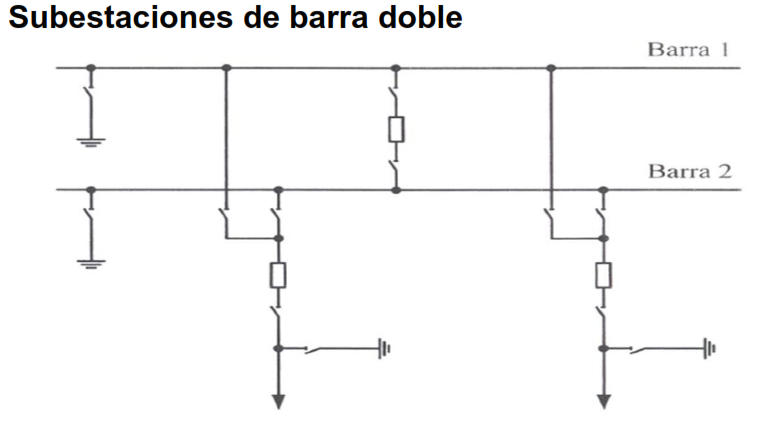
\includegraphics[scale = 0.6]{7.png}
    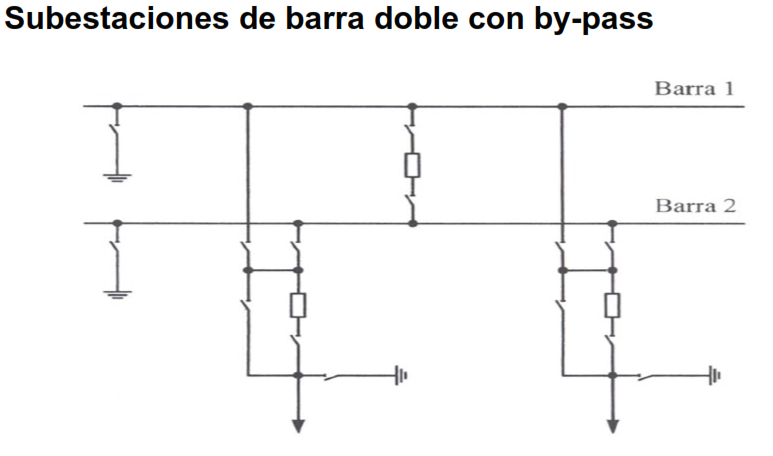
\includegraphics[scale = 0.6]{8.png}
    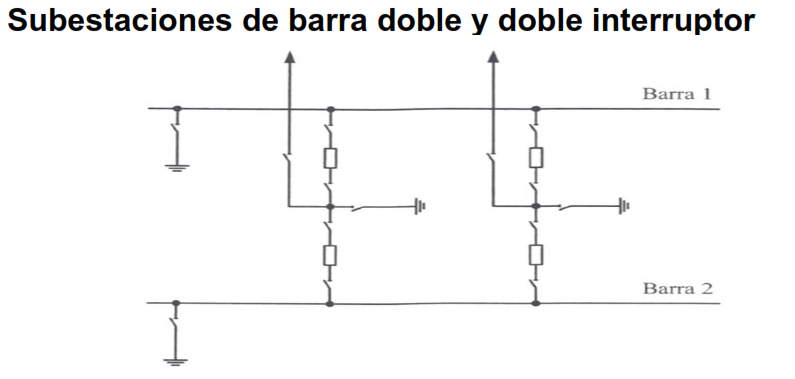
\includegraphics[scale = 0.6]{9.png}
    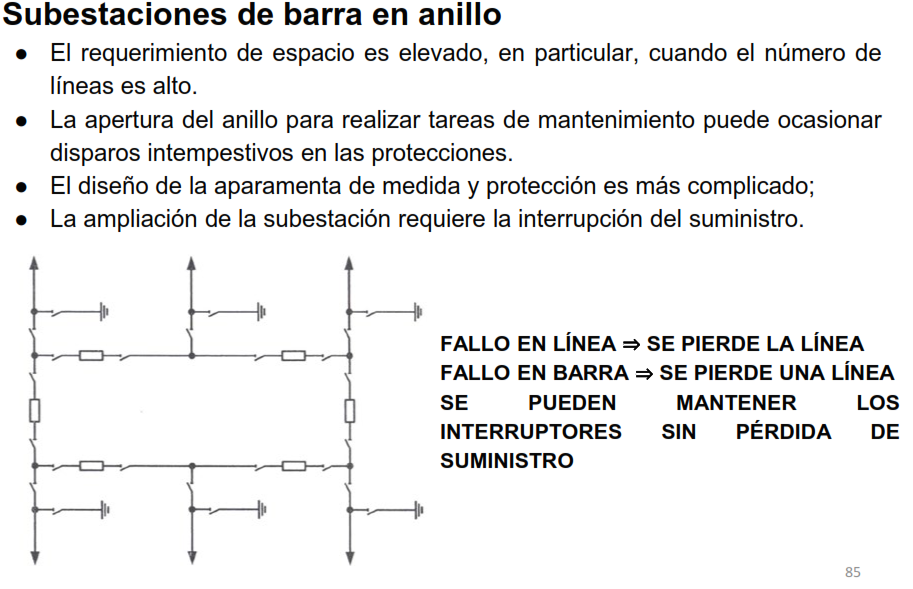
\includegraphics[scale = 0.6]{10.png}
    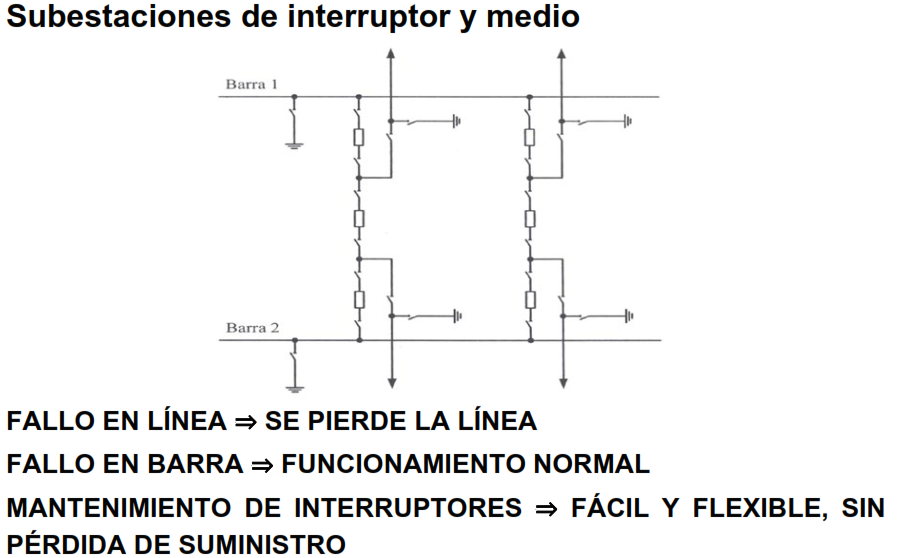
\includegraphics[scale = 0.6]{11.png}
\end{center}


\end{document}
